\documentclass[]{article}
\usepackage[]{amsmath,amssymb}
\usepackage{longtable}             % tables longer than one page - used for nomenclature
\usepackage{graphicx}    % needed for including graphics e.g. EPS, PS\begin{document}

\begin{document}

\section{Wishlist}
The purpose of this wishlist is to collect ideas on the implementation of usefull features in ACHP.

\subsection{Frontend//GUI}
\subsubsection{Display of the length of the different sections of the evaporator}
It would be nice to have a graph illustrating the length of the different sections
(subcooled, two-phase, superheated) of evaporator and condenser. Ideally it would be possible
to have 2 or 3 runs with different parameters plot into it to illustrate the influence
of e.g. an increase of charge.
  
\begin{figure}[htbp]
	\centering
		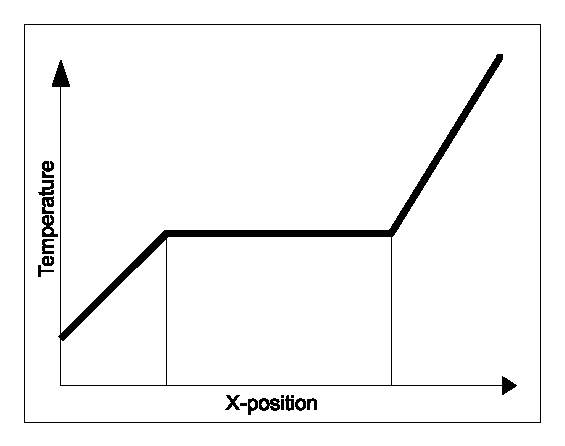
\includegraphics{wishlist_drawings_section_graph.eps}
	\label{fig:wishlist_drawings_section_graph}
	\caption{Graph showing sections of the evaporator}
\end{figure}


\subsection{Backend}
The current circuitry complexity assumption is neglected. It is wished to include the effect of different circuitry configuration on the performance of heat exchanger.
\end{document}
